\documentclass{article}

% ===== NeurIPS 2026 track =====
% PREPRINT (non-anonymous, arXiv-ready) -- used here for arXiv + peer/advisor review.
\PassOptionsToPackage{numbers, compress}{natbib}
\usepackage[preprint]{neurips_2026}
% For the ICBINB / NeurIPS WORKSHOP submission, comment the line above and use ONE of:
%   \usepackage[dblblindworkshop]{neurips_2026}   % double-blind (anonymise \author below)
%   \usepackage[sglblindworkshop]{neurips_2026}   % single-blind
% and set \workshoptitle{...}.

\usepackage[utf8]{inputenc}
\usepackage[T1]{fontenc}
\usepackage{hyperref}
\usepackage{url}
\usepackage{booktabs}
\usepackage{amsfonts}
\usepackage{amsmath}        % \binom, \text -- not in the NeurIPS default preamble
\usepackage{amssymb}        % \lesssim, \checkmark and other AMS symbols
\usepackage{nicefrac}
\usepackage{microtype}
\usepackage{xcolor}
\usepackage{pgfplots}
\pgfplotsset{compat=1.18}

% figures.tex --- preamble-safe figure setup, \input after the package preamble.
% Requires (already loaded in main.tex): \usepackage{pgfplots}; \pgfplotsset{compat=1.18}.
%
% This file holds ONLY preamble-safe declarations (no figure floats). The three
% figure floats live in fig_widens.tex, fig_wall.tex, and fig_degrade.tex and are
% \input at their placement points in the document body.

% pgfplots libraries used by the figures.
\usepgfplotslibrary{groupplots}

% TikZ libraries for the conceptual Figure 1 (capability matrix).
\usetikzlibrary{matrix,backgrounds,arrows.meta,positioning,fit,calc}

% Pass/fail glyphs for the dissociation matrix (\checkmark needs amssymb, loaded in main.tex).
\newcommand{\pass}{\textcolor{green!55!black}{\checkmark}}
\newcommand{\fail}{\textcolor{red!75!black}{\boldmath$\times$}}

% (No \begin{figure} content here: floats may not appear before \begin{document}.)


\title{Abduction: a reasoning axis where learned simulation and unaided frontier LLMs dissociate}
% \workshoptitle{WORKSHOP TITLE}   % required ONLY for the workshop tracks

\author{%
  Brian Sam-Bodden\thanks{Code and data: \url{https://github.com/integrallis/abduction-dissociation}} \\
  \texttt{bsbodden@gmail.com} \\
}

\begin{document}
\maketitle

\begin{abstract}
We study \emph{abduction}, the recovery of an unobserved initial condition from a noisy
trajectory, as a distinct axis of reasoning that sits alongside forward execution and
goal-directed control. We compare frontier LLMs, including the dedicated reasoning model o3,
against a deliberately non-transformer reasoner. That reasoner learns a world model from
black-box \texttt{(state, [action,] next-state)} transitions, never reading the true rule, and
reasons by simulating the model it learned. The inference is \textbf{simulation-based inference}
\cite{sbi2020}: maximum-a-posteriori (MAP) over forward rollouts. Our contribution is the
capability dissociation it exposes, not the method. A reasoning model closes forward
execution and interactive control; o3 solves Sokoban control 17/18, close to our 18/18. It does
not close abduction. As the trajectory grows the LLMs stay near the single-noisy-frame floor and collapse at long horizon,
while the learned-simulation reasoner tracks the true-dynamics recoverability oracle. At
cellular-automaton (CA) horizon 18, ours recovers 30/30 [0.88, 1.00], against o3 at 1/30 [0.01, 0.17] (4/30 at high effort) and Sonnet at 0/30
[0.00, 0.11], and the gap widens with difficulty. A second dedicated reasoning model from a different
lab (Claude Opus~4.8 in adaptive thinking) replicates the pattern in a smaller probe: it closes
forward and control yet does not reliably abduct. The failure is one of \emph{unaided} inference:
given code execution the same model writes the search and closes the gap (20/30, matching ours), which
points to in-context exact inverse search, rather than reasoning in general, as the bottleneck.
The learned model is load-bearing: recovery
follows its fidelity and falls to the floor when we degrade it, and the reasoner equals the
oracle. This is a forward/control-pass, inverse-fail \emph{dissociation} (o3 passes the axes it
shares with our reasoner and fails only the inverse one), and it holds across two structurally
different worlds, a reversible 1-D cellular automaton and an irreversible 2-D Sokoban.
\end{abstract}

\section{Introduction}
\label{sec:intro}

% FIGURE 1 --- the capability dissociation across the three reasoning axes.
% Conceptual "money figure": a 2x3 capability matrix with the abduction column
% highlighted, above a compact schematic of the three operations on a trajectory.
\begin{figure}[t]
  \centering
  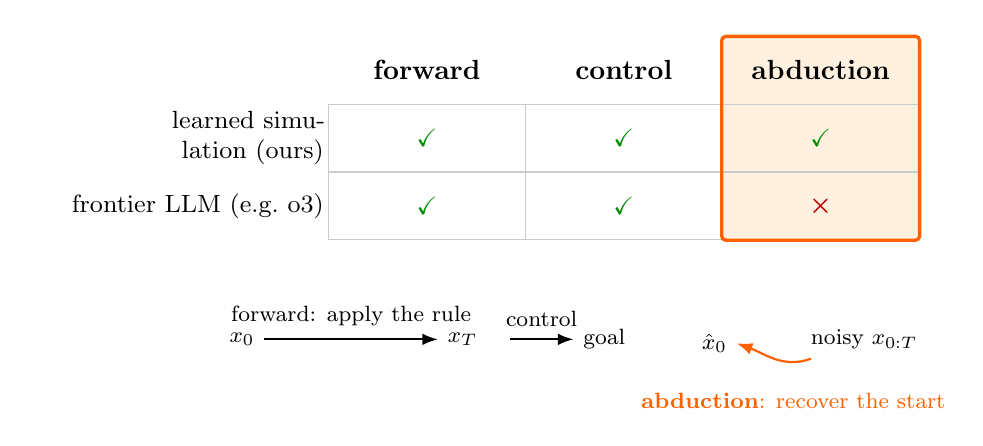
\begin{tikzpicture}[font=\small]
    % --- the capability matrix ---
    \matrix (m) [matrix of nodes,
        nodes={minimum width=2.5cm, minimum height=0.85cm, anchor=center,
               draw=gray!40, inner sep=3pt},
        column 1/.style={nodes={draw=none, text width=3.5cm, align=right}},
        row 1/.style={nodes={draw=none, font=\bfseries}},
        column sep=-\pgflinewidth, row sep=-\pgflinewidth]
    {
                                  & forward & control & abduction \\
      learned simulation (ours)   & \pass   & \pass   & \pass     \\
      frontier LLM (e.g.\ o3)     & \pass   & \pass   & \fail     \\
    };
    % shade + outline the abduction column (the gap, and the paper's subject)
    \begin{scope}[on background layer]
      \fill[orange!12] (m-1-4.north west) rectangle (m-3-4.south east);
    \end{scope}
    \draw[orange!75!red, very thick, rounded corners=1.5pt]
      (m-1-4.north west) rectangle (m-3-4.south east);

    % --- compact schematic of the three operations on a trajectory ---
    \begin{scope}[yshift=-2.55cm, font=\footnotesize]
      \node (x0) at (-3.0,0) {$x_0$};
      \node (xt) at (-0.2,0) {$x_T$};
      \draw[-{Latex[length=2mm]}, thick] (x0) -- (xt)
        node[midway, above=1pt] {forward: apply the rule};
      \node (g)  at (1.6,0) {goal};
      \draw[-{Latex[length=2mm]}, thick] (0.4,0) -- (g)
        node[midway, above=1pt] {control};
      % the inverse: a curved arrow running backward
      \node (obs) at (4.9,0) {noisy $x_{0:T}$};
      \node (xh)  at (3.0,-0.05) {$\hat{x}_0$};
      \draw[-{Latex[length=2mm]}, thick, orange!75!red]
        (obs) to[out=200,in=-20] (xh.east);
      \node[orange!75!red] at (4.0,-0.78) {\textbf{abduction}: recover the start};
    \end{scope}
  \end{tikzpicture}
  \caption{\textbf{The dissociation.} A reasoner can run a dynamical
  world \emph{forward}, \emph{control} it toward a target, or \emph{abduct} the initial
  condition from a noisy trajectory (the inverse). A frontier reasoning model (o3) closes
  the two forward-facing axes it shares with our learned-simulation reasoner, but not the
  inverse one. Our reasoner closes all three, sitting at the true-dynamics recoverability
  oracle. The orange column is the abduction gap.}
  \label{fig:dissociation}
\end{figure}


To reconstruct how a fire started, you reason backward from the wreckage to the spark. To predict
where a thrown ball will land, you run the world forward. These are different acts, and a mind can
be sharp at one and clumsy at the other. We show that frontier language models are lopsided in
exactly this way: they run a rule forward, and they intervene to steer it, but they cannot reliably
run it \emph{backward} to recover where a noisy trajectory began.

Most evaluations of reasoning in large language models hide this, because they collapse reasoning
into a single scalar on which one model is simply ``better at reasoning'' than another. We argue
instead that reasoning has distinguishable \emph{axes}, and that current frontier models pass some
while failing others in a way a scalar score conceals. Figure~\ref{fig:dissociation} summarizes the
result.

The core, after we cede the inference \emph{method} to simulation-based inference (SBI)
\cite{sbi2020} and the bare observation that ``LLMs fail backward'' to the reversal-curse literature
\cite{reversalcurse}, is a conjunction that, to our knowledge, no prior work draws. In plain terms: a
small non-transformer model learns the world's rule just by watching transitions, never being shown
it, and recovers a hidden starting state by simulating that learned rule forward and keeping the
candidate whose trajectory best matches the observation. Put to the same backward task, unaided
frontier LLMs pass forward execution and control yet fail the recovery; even a dedicated reasoning
model (o3) fails it, the gap grows with difficulty, and it holds in two structurally opposite worlds.
Formally:

\begin{quote}
a \textbf{non-transformer reasoner whose forward rule is learned from black-box transitions}
does initial-condition recovery by MAP-over-learned-rollouts, and this exposes a
\textbf{forward/control-pass, inverse-fail dissociation} in \emph{unaided} frontier LLMs that
\textbf{survives a dedicated reasoning model} (o3), with the gap \textbf{widening with
difficulty}, shown \textbf{unchanged across a reversible 1-D CA and an irreversible 2-D
Sokoban}.
\end{quote}

The conjunction is the contribution, and each element sets it beyond a nearby prior result: the
simulator is \emph{learned} from black-box transitions rather than given (beyond standard SBI); the
dissociation \emph{survives} a dedicated reasoning model (beyond the reversal curse); it holds
\emph{across} a reversible CA and an irreversible Sokoban (beyond a single domain); and the controls
show the learned model carries the inference, not a leaked oracle.

\paragraph{Scope, stated up front.}
The comparison is deliberately asymmetric, and we surface that here rather than only in
Section~\ref{sec:limitations}: our inverter is a \emph{hand-structured} simulator family (a
weight-shared local rule matched to each substrate, with exhaustive candidate search over small,
enumerable state spaces under a \emph{known} symmetric noise model), set against frontier LLMs
\emph{forbidden from writing or executing code}. The precise, well-supported reading is therefore not
that abduction is a new cognitive faculty, but that \emph{within this benchmark family} exact
initial-state recovery behaves as a \emph{separable} reasoning dimension on which unaided frontier
LLMs fail while a structured learned simulator succeeds up to a measured tractability wall. The gap is
a property of \emph{current unaided models as evaluated}, not a claim of architectural impossibility.

\paragraph{The three axes.}
We separate three things a reasoner can be asked to do over a dynamical world
(Table~\ref{tab:axes}). \emph{Forward execution} applies the rule $N$ steps. \emph{Control}, or
planning, finds $\leq B$ interventions that force a target state. \emph{Abduction} recovers the
initial condition from a noisy trajectory; it is the form of fault diagnosis, root-cause
analysis, forensic reconstruction, and scientific parameter inference, which all infer an unobserved
cause from its noisy consequences. The first two are gaps that separate weak models from
strong ones: o3 holds forward execution to $N{=}16$ where weak models fail by $N{=}4$, and it closes control (Sokoban 17/18,
against our 18/18 and Sonnet's 10/18). \textbf{Abduction is the axis o3 does not close} (CA
horizon-18: 1/30; Sokoban 5/8 $\rightarrow$ 2/8), while our reasoner sits at the oracle ceiling. We
measure that contrast on the \emph{same} worlds, with control as the matched within-domain
comparison, and that contrast is the contribution. o3 closes every axis it shares with our reasoner,
except the inverse one.

\begin{table}[t]
\centering
\caption{The three axes of reasoning. Forward and control are \emph{weak-LLM} gaps that a
dedicated reasoning model closes; abduction is the one it does not. The contrast is measured
on the same worlds, with control as the matched within-domain comparison.}
\label{tab:axes}
\begin{tabular}{@{}p{2.2cm}p{4.3cm}p{3.9cm}p{2.3cm}@{}}
\toprule
axis & what it tests & frontier-LLM behavior & our reasoner \\
\midrule
forward execution & apply the rule $N$ steps & o3 exact to $N{=}16$; weak LLMs fail by $N{=}4$ & exact \\
control / planning & find $\leq B$ interventions to force a target & o3 \textbf{closes} it (Sokoban 17/18) & 18/18 \\
\textbf{abduction} & recover the initial condition from a noisy trajectory & o3 \textbf{does not} close it (CA H=18: 1/30; Sokoban $n{=}8$: 5/8$\rightarrow$2/8) & oracle ceiling \\
\bottomrule
\end{tabular}
\end{table}

\section{The playgrounds}
\label{sec:domains}

We use two worlds chosen to be structurally opposite, so that a shared result cannot be a
single-domain artifact (Figure~\ref{fig:domains}).

\paragraph{A reversible 1-D cellular automaton.}
The first world is a ring of $L$ binary cells that updates in discrete time. An \emph{elementary}
cellular automaton sets each cell's next value from its three-cell neighborhood (left, self, right)
through a fixed Boolean lookup table; the eight possible neighborhoods give $2^8 = 256$ such tables,
and Wolfram's convention names each one by reading its eight outputs as an integer, hence ``Rule
110'' and ``Rule 90''. We use a \emph{second-order} lift, $\text{next}_i =
f(\text{cur}_{i-1},\text{cur}_i,\text{cur}_{i+1}) \oplus \text{prev}_i$, which is \emph{reversible}:
given $(\text{cur},\text{next})$ one recovers $\text{prev}$, so trajectories are well-posed in both
directions. A state is the pair $(\text{prev},\text{cur})$; an instance rolls a hidden initial
condition forward $T$ steps and reveals the trajectory under per-cell bit-flip noise.

The two rules matter because of \textbf{computational irreducibility}. \emph{Rule 110} is class-4
and Turing-complete: there is no closed form for its configuration at step $T$, so the only way to
know it is to run all $T$ steps, and inverting it therefore requires simulation.
\emph{Rule 90} is additive ($f(a,b,c) = a \oplus c$): it is linear, its evolution superposes, and
its step-$T$ state has a closed-form shortcut, visible as the regular Sierpinski triangle in
Figure~\ref{fig:domains}a. Rule 90 is our control. A method that ``solved'' the inverse only by
exploiting a shortcut would behave the same on both rules; a method that truly simulates should
behave differently, and ours does.

\paragraph{An irreversible 2-D Sokoban.}
The second world is Sokoban: an agent (the pusher) moves on a walled grid and shoves boxes onto
goal cells, one box per push, never pulling. Pushes are \emph{irreversible}: a box driven against a
wall cannot be undone. Unlike the CA, information about the past is genuinely destroyed. A
state is the grid layout (walls, boxes, pusher); an instance rolls a hidden initial layout forward
by a sequence of moves and reveals it under noise. Scoring in both worlds is exact: a recovered
initial condition counts only if every bit, or every cell, matches.

% FIGURE --- the two playgrounds: the CA (space-time, irreducible 110 vs reducible 90)
% and Sokoban. CA grids are REAL second-order traces (pce/ca/env.py), seed shown.
\begin{figure}[t]
  \centering
  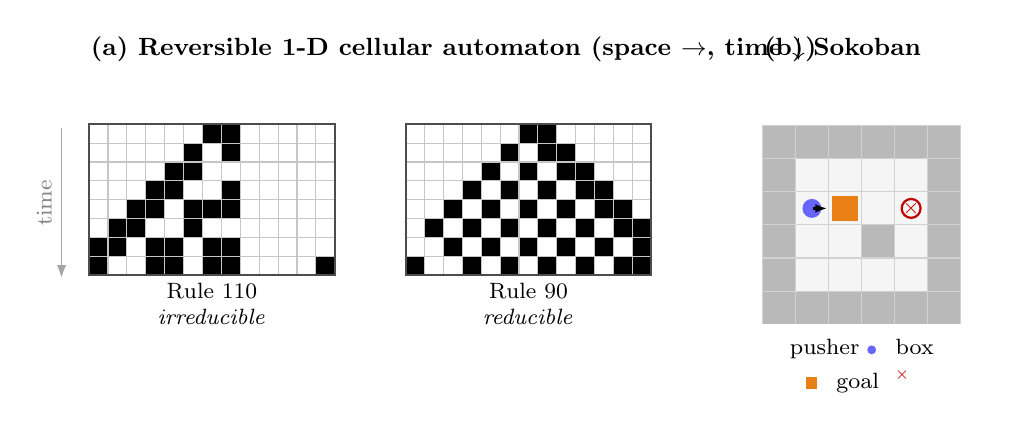
\begin{tikzpicture}[font=\small]
    % ---------- (a) Cellular automaton: two real space-time traces ----------
    \node[anchor=west, font=\small\bfseries] at (-0.1,0.95) {(a) Reversible 1-D cellular automaton (space $\rightarrow$, time $\downarrow$)};
    \draw[-{Latex[length=1.6mm]}, gray!70] (-0.35,-0.05) -- (-0.35,-1.95) node[midway,rotate=90,anchor=south,font=\footnotesize,gray] {time};
    % Rule 110 space-time
    \begin{scope}[xshift=0.00cm]
    \fill[black] (1.44,0.00) rectangle (1.68,-0.24);
    \fill[black] (1.68,0.00) rectangle (1.92,-0.24);
    \fill[black] (1.20,-0.24) rectangle (1.44,-0.48);
    \fill[black] (1.68,-0.24) rectangle (1.92,-0.48);
    \fill[black] (0.96,-0.48) rectangle (1.20,-0.72);
    \fill[black] (1.20,-0.48) rectangle (1.44,-0.72);
    \fill[black] (0.72,-0.72) rectangle (0.96,-0.96);
    \fill[black] (0.96,-0.72) rectangle (1.20,-0.96);
    \fill[black] (1.68,-0.72) rectangle (1.92,-0.96);
    \fill[black] (0.48,-0.96) rectangle (0.72,-1.20);
    \fill[black] (0.72,-0.96) rectangle (0.96,-1.20);
    \fill[black] (1.20,-0.96) rectangle (1.44,-1.20);
    \fill[black] (1.44,-0.96) rectangle (1.68,-1.20);
    \fill[black] (1.68,-0.96) rectangle (1.92,-1.20);
    \fill[black] (0.24,-1.20) rectangle (0.48,-1.44);
    \fill[black] (0.48,-1.20) rectangle (0.72,-1.44);
    \fill[black] (1.20,-1.20) rectangle (1.44,-1.44);
    \fill[black] (0.00,-1.44) rectangle (0.24,-1.68);
    \fill[black] (0.24,-1.44) rectangle (0.48,-1.68);
    \fill[black] (0.72,-1.44) rectangle (0.96,-1.68);
    \fill[black] (0.96,-1.44) rectangle (1.20,-1.68);
    \fill[black] (1.44,-1.44) rectangle (1.68,-1.68);
    \fill[black] (1.68,-1.44) rectangle (1.92,-1.68);
    \fill[black] (0.00,-1.68) rectangle (0.24,-1.92);
    \fill[black] (0.72,-1.68) rectangle (0.96,-1.92);
    \fill[black] (0.96,-1.68) rectangle (1.20,-1.92);
    \fill[black] (1.44,-1.68) rectangle (1.68,-1.92);
    \fill[black] (1.68,-1.68) rectangle (1.92,-1.92);
    \fill[black] (2.88,-1.68) rectangle (3.12,-1.92);
    \draw[gray!45] (0,0) grid[step=0.24cm] (3.12,-1.92);
    \draw[black!70, thick] (0,0) rectangle (3.12,-1.92);
    \node[font=\footnotesize, align=center] at (1.56,-2.28) {Rule 110\\ \emph{irreducible}};
    \end{scope}
    % Rule 90 space-time
    \begin{scope}[xshift=4.02cm]
    \fill[black] (1.44,0.00) rectangle (1.68,-0.24);
    \fill[black] (1.68,0.00) rectangle (1.92,-0.24);
    \fill[black] (1.20,-0.24) rectangle (1.44,-0.48);
    \fill[black] (1.68,-0.24) rectangle (1.92,-0.48);
    \fill[black] (1.92,-0.24) rectangle (2.16,-0.48);
    \fill[black] (0.96,-0.48) rectangle (1.20,-0.72);
    \fill[black] (1.44,-0.48) rectangle (1.68,-0.72);
    \fill[black] (1.92,-0.48) rectangle (2.16,-0.72);
    \fill[black] (2.16,-0.48) rectangle (2.40,-0.72);
    \fill[black] (0.72,-0.72) rectangle (0.96,-0.96);
    \fill[black] (1.20,-0.72) rectangle (1.44,-0.96);
    \fill[black] (1.68,-0.72) rectangle (1.92,-0.96);
    \fill[black] (2.16,-0.72) rectangle (2.40,-0.96);
    \fill[black] (2.40,-0.72) rectangle (2.64,-0.96);
    \fill[black] (0.48,-0.96) rectangle (0.72,-1.20);
    \fill[black] (0.96,-0.96) rectangle (1.20,-1.20);
    \fill[black] (1.44,-0.96) rectangle (1.68,-1.20);
    \fill[black] (1.92,-0.96) rectangle (2.16,-1.20);
    \fill[black] (2.40,-0.96) rectangle (2.64,-1.20);
    \fill[black] (2.64,-0.96) rectangle (2.88,-1.20);
    \fill[black] (0.24,-1.20) rectangle (0.48,-1.44);
    \fill[black] (0.72,-1.20) rectangle (0.96,-1.44);
    \fill[black] (1.20,-1.20) rectangle (1.44,-1.44);
    \fill[black] (1.68,-1.20) rectangle (1.92,-1.44);
    \fill[black] (2.16,-1.20) rectangle (2.40,-1.44);
    \fill[black] (2.64,-1.20) rectangle (2.88,-1.44);
    \fill[black] (2.88,-1.20) rectangle (3.12,-1.44);
    \fill[black] (0.48,-1.44) rectangle (0.72,-1.68);
    \fill[black] (0.96,-1.44) rectangle (1.20,-1.68);
    \fill[black] (1.44,-1.44) rectangle (1.68,-1.68);
    \fill[black] (1.92,-1.44) rectangle (2.16,-1.68);
    \fill[black] (2.40,-1.44) rectangle (2.64,-1.68);
    \fill[black] (2.88,-1.44) rectangle (3.12,-1.68);
    \fill[black] (0.00,-1.68) rectangle (0.24,-1.92);
    \fill[black] (0.72,-1.68) rectangle (0.96,-1.92);
    \fill[black] (1.20,-1.68) rectangle (1.44,-1.92);
    \fill[black] (1.68,-1.68) rectangle (1.92,-1.92);
    \fill[black] (2.16,-1.68) rectangle (2.40,-1.92);
    \fill[black] (2.64,-1.68) rectangle (2.88,-1.92);
    \fill[black] (2.88,-1.68) rectangle (3.12,-1.92);
    \draw[gray!45] (0,0) grid[step=0.24cm] (3.12,-1.92);
    \draw[black!70, thick] (0,0) rectangle (3.12,-1.92);
    \node[font=\footnotesize, align=center] at (1.56,-2.28) {Rule 90\\ \emph{reducible}};
    \end{scope}

    % ---------- (b) Sokoban board ----------
    \begin{scope}[xshift=8.55cm, yshift=-0.02cm]
      \def\cs{0.42}
      \node[anchor=west, font=\small\bfseries] at (-0.1,0.97) {(b) Sokoban};
      \fill[gray!8] (0,0) rectangle (6*\cs,-6*\cs);
      \foreach \x in {0,...,5}{\fill[gray!55] (\x*\cs,0) rectangle ({(\x+1)*\cs},-\cs);
        \fill[gray!55] (\x*\cs,-5*\cs) rectangle ({(\x+1)*\cs},-6*\cs);}
      \foreach \y in {0,...,5}{\fill[gray!55] (0,-\y*\cs) rectangle (\cs,{-(\y+1)*\cs});
        \fill[gray!55] (5*\cs,-\y*\cs) rectangle (6*\cs,{-(\y+1)*\cs});}
      \fill[gray!55] (3*\cs,-3*\cs) rectangle (4*\cs,-4*\cs);                       % interior wall
      \draw[red!75!black, thick] ({4*\cs+\cs/2},{-2*\cs-\cs/2}) circle (0.12);       % goal
      \node[red!75!black, font=\scriptsize] at ({4*\cs+\cs/2},{-2*\cs-\cs/2}) {$\times$};
      \fill[orange!65!brown] ({2*\cs+0.05},{-2*\cs-0.05}) rectangle ({3*\cs-0.05},{-3*\cs+0.05}); % box
      \fill[blue!60] ({1*\cs+\cs/2},{-2*\cs-\cs/2}) circle (0.12);                  % pusher
      \draw[-{Latex[length=1.5mm]}, thick] ({1.52*\cs},{-2.5*\cs}) -- ({1.96*\cs},{-2.5*\cs}); % push
      \draw[gray!35] (0,0) grid[step=\cs cm] (6*\cs,-6*\cs);
      \node[font=\footnotesize, align=center, text width=2.9cm] at (3*\cs,-3.05) {pusher \tikz\fill[blue!60] circle(1.6pt); \, box \tikz\fill[orange!65!brown](0,0)rectangle(4pt,4pt); \, goal \tikz\node[red!75!black,font=\tiny]{$\times$};};
    \end{scope}
  \end{tikzpicture}
  \caption{\textbf{The two playgrounds.} \textbf{(a)} Real space-time traces of the
  second-order CA from one seed (width-13 ring shown; the rule is width-independent). Each row
  is one configuration; time runs down. \emph{Rule 110} (left) is computationally
  \emph{irreducible} (class-4, Turing-complete): its irregular pattern cannot be predicted
  faster than by simulating every step. \emph{Rule 90} (right) is \emph{reducible} (additive,
  $f(a,b,c)=a\oplus c$): the regular Sierpinski structure means a closed-form shortcut exists,
  so it is our control. \textbf{(b)} A Sokoban instance: a pusher moves on a walled grid and
  shoves boxes onto goals. Pushes are \emph{irreversible} (a box shoved against a wall cannot
  be pulled back), so this world is structurally unlike the reversible CA.}
  \label{fig:domains}
\end{figure}


\section{The reasoner}
\label{sec:method}

The reasoner never reads the rule. It learns a forward model from black-box transitions, then
inverts that model by simulation. This is \textbf{simulation-based
inference} (SBI) \cite{sbi2020}: recover a latent input by rolling a forward simulator and scoring
against the observation. The one thing we add is that the simulator is \emph{learned from black-box
transitions}, with no rule access; the other is the head-to-head against LLMs across the three axes.
Figure~\ref{fig:reasoner} and Algorithm~1 give the mechanism in full.

\paragraph{The learned forward model.}
The model is a single \textbf{weight-shared local rule} $f_\theta$: a small MLP that maps one
cell's neighborhood $(\text{prev}_i, \text{cur}_{i-1}, \text{cur}_i, \text{cur}_{i+1})$ to that
cell's next value, applied identically at every cell and every ring width. Because no width
parameter appears in the weights, a model fit on small rings instantiates unchanged on larger ones,
so size-generalization is structural rather than hoped for. The model reads neither the rule code nor
the width; the training details (architecture, optimizer, data) are in Section~\ref{sec:setup}.

\paragraph{Abduction as MAP over learned rollouts.}
Given a noisy trajectory, the reasoner enumerates candidate initial conditions, rolls each one
forward $T$ steps under $f_\theta$, scores the simulated trajectory against the observation by a
per-cell likelihood, and returns the maximum-a-posteriori candidate (Algorithm~1).
Evidence is aggregated across the \emph{whole} trajectory, and that aggregation is the inference.
The inverse problem is not hard once the rule is known; it is classical pre-image computation. The
contribution is the learned substrate and the dissociation it exposes.

\begin{figure}[t]
\centering
\begin{minipage}{0.96\linewidth}
\hrule\vspace{2.5pt}
{\small\textbf{Algorithm 1}\quad MAP abduction over the learned model}\vspace{2.5pt}
\hrule\vspace{4pt}
{\small
\textbf{Require:} noisy trajectory $\tilde{y}_{0:T}$;\ learned rule $f_\theta$;\ candidate set $\mathcal{X}_0$\\[2pt]
1:\quad $\text{best} \gets -\infty$;\ \ $\hat{x}_0 \gets \varnothing$\\
2:\quad \textbf{for} each candidate $x_0 \in \mathcal{X}_0$ \textbf{do}\\
3:\quad\quad $\hat{y}_{0:T} \gets \textsc{Rollout}(f_\theta,\, x_0,\, T)$ \hfill $\triangleright$ simulate the \emph{learned} model, never the true one\\
4:\quad\quad $\ell \gets \sum_{t=0}^{T}\sum_i \log p(\tilde{y}_{t,i} \mid \hat{y}_{t,i})$ \hfill $\triangleright$ whole-trajectory per-cell log-likelihood\\
5:\quad\quad \textbf{if} $\ell > \text{best}$ \textbf{then} $\text{best} \gets \ell$;\ \ $\hat{x}_0 \gets x_0$\\
6:\quad \textbf{return} $\hat{x}_0$
}\vspace{4pt}
\hrule
\end{minipage}
\end{figure}

% FIGURE --- the reasoner mechanism: learn a forward model from black-box
% transitions (top), then invert it by MAP over learned rollouts (bottom).
\begin{figure}[t]
  \centering
  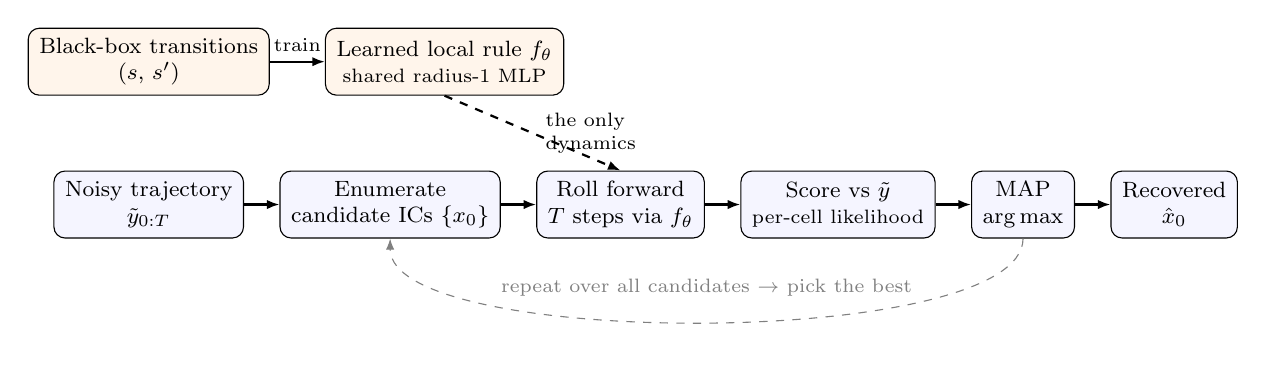
\begin{tikzpicture}[font=\footnotesize, >={Latex[length=1.6mm]},
      box/.style={draw, rounded corners, align=center, inner xsep=4pt, inner ysep=3pt,
                  minimum height=0.85cm, fill=blue!4},
      tbox/.style={draw, rounded corners, align=center, inner xsep=4pt, inner ysep=3pt,
                   minimum height=0.85cm, fill=orange!8},
      ar/.style={->, thick}]
    % --- training path (top) ---
    \node[tbox] (tr) {Black-box transitions\\$(s,\,s')$};
    \node[tbox, right=0.7cm of tr] (rule) {Learned local rule $f_\theta$\\{\scriptsize shared radius-1 MLP}};
    \draw[ar] (tr) -- (rule) node[midway, above, font=\scriptsize] {train};
    % --- abduction path (bottom) ---
    \node[box, below=0.95cm of tr] (obs) {Noisy trajectory\\$\tilde{y}_{0:T}$};
    \node[box, right=0.45cm of obs] (enum) {Enumerate\\candidate ICs $\{x_0\}$};
    \node[box, right=0.45cm of enum] (sim) {Roll forward\\$T$ steps via $f_\theta$};
    \node[box, right=0.45cm of sim] (score) {Score vs $\tilde{y}$\\{\scriptsize per-cell likelihood}};
    \node[box, right=0.45cm of score] (map) {MAP\\$\arg\max$};
    \node[box, right=0.45cm of map] (out) {Recovered\\$\hat{x}_0$};
    \draw[ar] (obs) -- (enum);
    \draw[ar] (enum) -- (sim);
    \draw[ar] (sim) -- (score);
    \draw[ar] (score) -- (map);
    \draw[ar] (map) -- (out);
    % the learned model is the ONLY dynamics used in the loop
    \draw[ar, dashed] (rule.south) -- (sim.north)
      node[midway, right=1pt, font=\scriptsize, align=left] {the only\\dynamics};
    % the iteration: a loop-back arrow BELOW the row, clear of the dashed dynamics arrow above
    \draw[->, dashed, gray, >={Latex[length=1.4mm]}] (map.south) to[out=-90, in=-90, looseness=0.45] (enum.south);
    \node[font=\scriptsize, gray] at ($(enum.south)!0.5!(map.south)+(0,-0.62)$) {repeat over all candidates $\rightarrow$ pick the best};
  \end{tikzpicture}
  \caption{\textbf{The reasoner.} A forward model is \emph{learned} from black-box
  \texttt{(state, [action,] next-state)} transitions (top): one weight-shared radius-1 rule $f_\theta$,
  applied at every cell and every system size, so it generalizes across width by construction.
  Abduction (bottom) is maximum-a-posteriori inference over that learned model: enumerate
  candidate initial conditions, roll each one forward under $f_\theta$, score the simulated
  trajectory against the noisy observation, and return the best (Algorithm~1).
  The true environment is never queried during the search; $f_\theta$ supplies all dynamics.}
  \label{fig:reasoner}
\end{figure}


\section{Experimental setup}
\label{sec:setup}

\paragraph{Instances and the noise channel.}
A CA instance draws a hidden initial condition $x_0 = (\text{prev}_0, \text{cur}_0)$ uniformly from
$\{0,1\}^L \times \{0,1\}^L$, rolls it forward $H$ steps under the true rule (the horizon $H$ is the
$T$ of Algorithm~1), and reveals all $H{+}1$
frames through an i.i.d.\ bit-flip channel: every cell is flipped independently with probability
$\eta$ (we use $\eta = 0.2$). Sokoban noises only the box and agent cells, leaving walls and goals
intact, so the static board is read from the first frame. Unless stated otherwise the CA runs at
$L=8$, $H \in \{6,12,18\}$; size generalization is tested at $L \in \{11,12\}$, both outside the
$L \le 10$ training range. Scoring is exact: a recovered initial condition (IC) counts only if it matches the truth in
every bit (CA) or cell (Sokoban).

\paragraph{Likelihood, prior, candidate set, and oracle.}
Under the symmetric channel the per-cell likelihood is $p(\tilde y \mid \hat y) =
(1-\eta)^{[\tilde y = \hat y]}\,\eta^{[\tilde y \ne \hat y]}$, so with a uniform prior over
$\mathcal{X}_0$ the MAP of Algorithm~1 reduces to the candidate whose rollout agrees with the
observation in the most cells. The candidate set $\mathcal{X}_0$ is, for the CA, all $2^{2L}$ pairs
$(\text{prev}, \text{cur})$ (enumerated exhaustively; feasible to $L \approx 12$, Section~\ref{sec:limitations});
for Sokoban, the $\binom{\text{free}}{k}(\text{free}-k)$ placements of the $k{=}2$ boxes and the
pusher over free cells, with walls and goals held to their observed positions. Ties take the lowest
index. The \textbf{recoverability oracle} is Algorithm~1 run with the \emph{true} rule in place of
$f_\theta$ (same $\mathcal{X}_0$, likelihood, and noise draw); it is the best exact recovery the noise
allows, so ``ours $=$ oracle'' means the learned model loses nothing to the true one.

\paragraph{The learned model.}
$f_\theta$ is a two-layer MLP ($4 \to 16 \to 1$, ReLU), trained by binary cross-entropy (Adam, learning
rate $0.01$, $1500$ steps, batch $512$) on black-box \texttt{(state, next-state)} transitions pooled
over widths $\{6,7,8,9,10\}$ ($400$ per width); the predicted bit is $\text{logit} > 0$.
\emph{Fidelity} (the degrade control, Section~\ref{sec:controls}) is its held-out one-step
whole-configuration exact-match rate, dialed by the training-step budget. \emph{Exact joint recovery}
(the main metric) is the per-instance indicator that the recovered $\hat x_0$ matches the true $x_0$
in every bit.

\paragraph{LLM baselines and the evaluation protocol.}
We compare a dedicated reasoning model (o3, \texttt{reasoning\_effort=medium}, with a high-effort
robustness run), a \emph{second} dedicated reasoning model from a different lab (Claude Opus~4.8 in
adaptive/extended thinking, a smaller $n=5$/cell probe), a frontier chat model (Claude Sonnet~4.6),
and, on the forward axis, a deliberately weak model (GPT-4o-mini). Decoding is temperature $0$, up to
$8192$ tokens for the o-series and chat models. For the adaptive-thinking model the chain-of-thought
counts against the output cap, so we raise it to the $128$k ceiling and log \texttt{stop\_reason}; an
instance whose thinking overruns even $128$k is re-run at lower effort, never scored on a truncated
trace. Each model is
handed the \emph{exact rule table}, the dynamics equation, and the noise level in-prompt and may use a
scratchpad; tools and code execution are disallowed, since writing the inversion program is retrieval
of a known algorithm, not abduction. Answers must end in fixed tags (e.g.\ \texttt{FINAL\_X0} /
\texttt{FINAL\_X1}); extraction is strict and we report the \textbf{parse rate}, so a malformed answer
is never scored as a reasoning failure (Appendix~\ref{app:prompts}). Sample sizes: CA ours
$n{=}200$/rule over $5$ seeds, CA LLMs $n{=}15$/rule/horizon; Sokoban ours $n{=}36$/size over $3$
seeds, LLMs $n{=}8$. Code and the cached LLM transcripts are released with the paper.

\section{Results}
\label{sec:results}

\subsection{Cellular automaton: the abduction gap, and it widens}

% FIGURE --- a worked abduction instance: real Rule-110, L=8, H=8, noise 0.2, seed 2.
% The reasoner sees only the noisy trajectory (12/72 bits flipped) and recovers (x0,x1) exactly.
\begin{figure}[t]
  \centering
  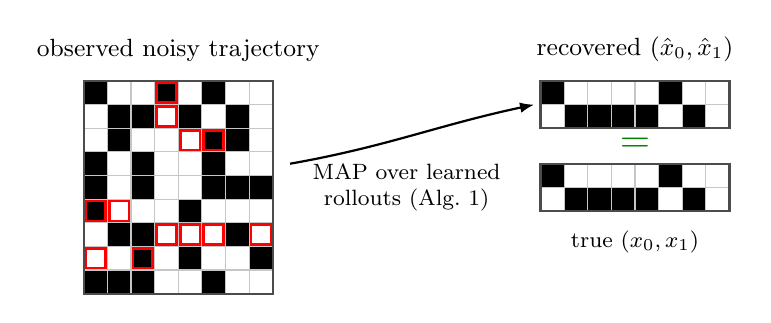
\begin{tikzpicture}[font=\footnotesize, >={Latex[length=1.8mm]}]
    \node[anchor=south, font=\small] at (1.2,0.12) {observed noisy trajectory};
  \fill[black] (0.00,0.00) rectangle (0.30,-0.30);
  \fill[black] (0.90,0.00) rectangle (1.20,-0.30);
  \fill[black] (1.50,0.00) rectangle (1.80,-0.30);
  \fill[black] (0.30,-0.30) rectangle (0.60,-0.60);
  \fill[black] (0.60,-0.30) rectangle (0.90,-0.60);
  \fill[black] (1.20,-0.30) rectangle (1.50,-0.60);
  \fill[black] (1.80,-0.30) rectangle (2.10,-0.60);
  \fill[black] (0.30,-0.60) rectangle (0.60,-0.90);
  \fill[black] (1.50,-0.60) rectangle (1.80,-0.90);
  \fill[black] (1.80,-0.60) rectangle (2.10,-0.90);
  \fill[black] (0.00,-0.90) rectangle (0.30,-1.20);
  \fill[black] (0.60,-0.90) rectangle (0.90,-1.20);
  \fill[black] (1.50,-0.90) rectangle (1.80,-1.20);
  \fill[black] (0.00,-1.20) rectangle (0.30,-1.50);
  \fill[black] (0.60,-1.20) rectangle (0.90,-1.50);
  \fill[black] (1.50,-1.20) rectangle (1.80,-1.50);
  \fill[black] (1.80,-1.20) rectangle (2.10,-1.50);
  \fill[black] (2.10,-1.20) rectangle (2.40,-1.50);
  \fill[black] (0.00,-1.50) rectangle (0.30,-1.80);
  \fill[black] (1.20,-1.50) rectangle (1.50,-1.80);
  \fill[black] (0.30,-1.80) rectangle (0.60,-2.10);
  \fill[black] (0.60,-1.80) rectangle (0.90,-2.10);
  \fill[black] (1.80,-1.80) rectangle (2.10,-2.10);
  \fill[black] (0.60,-2.10) rectangle (0.90,-2.40);
  \fill[black] (1.20,-2.10) rectangle (1.50,-2.40);
  \fill[black] (2.10,-2.10) rectangle (2.40,-2.40);
  \fill[black] (0.00,-2.40) rectangle (0.30,-2.70);
  \fill[black] (0.30,-2.40) rectangle (0.60,-2.70);
  \fill[black] (0.60,-2.40) rectangle (0.90,-2.70);
  \fill[black] (1.50,-2.40) rectangle (1.80,-2.70);
  \draw[red,very thick] (0.92,-0.02) rectangle (1.18,-0.28);
  \draw[red,very thick] (0.92,-0.32) rectangle (1.18,-0.58);
  \draw[red,very thick] (1.22,-0.62) rectangle (1.48,-0.88);
  \draw[red,very thick] (1.52,-0.62) rectangle (1.78,-0.88);
  \draw[red,very thick] (0.02,-1.52) rectangle (0.28,-1.78);
  \draw[red,very thick] (0.32,-1.52) rectangle (0.58,-1.78);
  \draw[red,very thick] (0.92,-1.82) rectangle (1.18,-2.08);
  \draw[red,very thick] (1.22,-1.82) rectangle (1.48,-2.08);
  \draw[red,very thick] (1.52,-1.82) rectangle (1.78,-2.08);
  \draw[red,very thick] (2.12,-1.82) rectangle (2.38,-2.08);
  \draw[red,very thick] (0.02,-2.12) rectangle (0.28,-2.38);
  \draw[red,very thick] (0.62,-2.12) rectangle (0.88,-2.38);
  \draw[gray!45] (0,0) grid[step=0.3cm] (2.40,-2.70);
  \draw[black!70,thick] (0,0) rectangle (2.40,-2.70);
    % MAP arrow
    \draw[->,thick] (2.62,-1.05) to[out=10,in=192] (5.72,-0.30);
    \node[font=\footnotesize, align=center] at (4.10,-1.35) {MAP over learned\\rollouts (Alg.~1)};
    \begin{scope}[xshift=1.4cm]
    \node[anchor=south, font=\small] at (5.6,0.12) {recovered $(\hat{x}_0,\hat{x}_1)$};
  \fill[black] (4.40,0.00) rectangle (4.70,-0.30);
  \fill[black] (5.90,0.00) rectangle (6.20,-0.30);
  \draw[gray!45] (4.40,0.00) rectangle (6.80,-0.30);
  \draw[gray!45] (4.70,0.00) rectangle (5.00,-0.30);
  \draw[gray!45] (5.00,0.00) rectangle (5.30,-0.30);
  \draw[gray!45] (5.30,0.00) rectangle (5.60,-0.30);
  \draw[gray!45] (5.60,0.00) rectangle (5.90,-0.30);
  \draw[gray!45] (5.90,0.00) rectangle (6.20,-0.30);
  \draw[gray!45] (6.20,0.00) rectangle (6.50,-0.30);
  \fill[black] (4.70,-0.30) rectangle (5.00,-0.60);
  \fill[black] (5.00,-0.30) rectangle (5.30,-0.60);
  \fill[black] (5.30,-0.30) rectangle (5.60,-0.60);
  \fill[black] (5.60,-0.30) rectangle (5.90,-0.60);
  \fill[black] (6.20,-0.30) rectangle (6.50,-0.60);
  \draw[gray!45] (4.40,-0.30) rectangle (6.80,-0.60);
  \draw[gray!45] (4.70,-0.30) rectangle (5.00,-0.60);
  \draw[gray!45] (5.00,-0.30) rectangle (5.30,-0.60);
  \draw[gray!45] (5.30,-0.30) rectangle (5.60,-0.60);
  \draw[gray!45] (5.60,-0.30) rectangle (5.90,-0.60);
  \draw[gray!45] (5.90,-0.30) rectangle (6.20,-0.60);
  \draw[gray!45] (6.20,-0.30) rectangle (6.50,-0.60);
  \draw[black!70,thick] (4.40,0.00) rectangle (6.80,-0.60);
    \node[anchor=north, font=\footnotesize] at (5.6,-1.78) {true $(x_0,x_1)$};
  \fill[black] (4.40,-1.05) rectangle (4.70,-1.35);
  \fill[black] (5.90,-1.05) rectangle (6.20,-1.35);
  \draw[gray!45] (4.40,-1.05) rectangle (6.80,-1.35);
  \draw[gray!45] (4.70,-1.05) rectangle (5.00,-1.35);
  \draw[gray!45] (5.00,-1.05) rectangle (5.30,-1.35);
  \draw[gray!45] (5.30,-1.05) rectangle (5.60,-1.35);
  \draw[gray!45] (5.60,-1.05) rectangle (5.90,-1.35);
  \draw[gray!45] (5.90,-1.05) rectangle (6.20,-1.35);
  \draw[gray!45] (6.20,-1.05) rectangle (6.50,-1.35);
  \fill[black] (4.70,-1.35) rectangle (5.00,-1.65);
  \fill[black] (5.00,-1.35) rectangle (5.30,-1.65);
  \fill[black] (5.30,-1.35) rectangle (5.60,-1.65);
  \fill[black] (5.60,-1.35) rectangle (5.90,-1.65);
  \fill[black] (6.20,-1.35) rectangle (6.50,-1.65);
  \draw[gray!45] (4.40,-1.35) rectangle (6.80,-1.65);
  \draw[gray!45] (4.70,-1.35) rectangle (5.00,-1.65);
  \draw[gray!45] (5.00,-1.35) rectangle (5.30,-1.65);
  \draw[gray!45] (5.30,-1.35) rectangle (5.60,-1.65);
  \draw[gray!45] (5.60,-1.35) rectangle (5.90,-1.65);
  \draw[gray!45] (5.90,-1.35) rectangle (6.20,-1.65);
  \draw[gray!45] (6.20,-1.35) rectangle (6.50,-1.65);
  \draw[black!70,thick] (4.40,-1.05) rectangle (6.80,-1.65);
    \node[green!50!black, font=\Large\bfseries] at (5.60,-0.82) {$=$};
    \end{scope}
  \end{tikzpicture}
  \caption{\textbf{A worked instance.} A hidden Rule-110 initial condition is rolled forward $H=8$
  steps and revealed through the bit-flip channel, which flips \textbf{12 of the 72 bits} (red
  outlines). From this noisy trajectory alone, the reasoner's MAP over learned rollouts
  (Algorithm~1) recovers the true first two rows $(x_0, x_1)$ \emph{exactly}: the recovered pair
  (upper right) equals the truth (lower right). $L=8$, noise $0.2$, seed 2.}
  \label{fig:example}
\end{figure}


Figure~\ref{fig:example} shows one instance: from a trajectory with 12 of its 72 bits flipped, the
reasoner recovers the hidden IC exactly. In aggregate, our learned-model MAP is pinned to the
true-dynamics recoverability oracle at every difficulty, across 5 seeds, $n=200$/rule. Ours equals the true-dynamics MAP at every (rule, noise),
and ours falls only where the \emph{oracle ceiling} itself falls, to task ambiguity, never below it.
The reasoner is therefore not under-performing. Where exact recovery drops, the ceiling drops with
it.

This recovery generalizes across width. Trained only on $L \le 10$, the same rule abducts at unseen
widths $L=11$ ($57/60$ and $55/60$ for Rules 110 and 90) and $L=12$ ($58/60$, $49/60$), matching the
oracle at every cell: size generalization, not in-distribution reuse.

The gap to the LLMs grows with difficulty rather than shrinking: it
\emph{widens with trajectory length} ($n=15$/rule across horizons $H \in \{6,12,18\}$, transcripts
cached). Figure~\ref{fig:widens} plots exact joint recovery, pooled over both rules ($n=30$/cell). At
$H=6$, ours is $0.467$, o3 $0.100$, Sonnet $0.000$; at $H=12$, ours $0.733$, o3 $0.167$, Sonnet
$0.033$; at $H=18$, ours $1.000$, o3 $0.033$, Sonnet $0.000$. Pooled at $H=18$, ours recovers 30/30
[0.88, 1.00] against o3 at 1/30 [0.01, 0.17] and Sonnet at 0/30 [0.00, 0.11], with non-overlapping
Wilson 95\% intervals. Because the design reuses seeded instances, the comparison is \emph{paired}: an
exact McNemar test over all matched instances rejects equality decisively (ours vs o3
$p=1.4\times10^{-17}$, vs Sonnet $p=5.4\times10^{-20}$; ours vs Opus~4.8 $p<10^{-3}$), and ours never
loses a discordant instance to any LLM ($c=0$ throughout; \texttt{experiments/significance.py}). The gap is not an effort artifact: at \texttt{reasoning\_effort=high} o3 still
reaches only $4/30$ (parse rate $27/30$, so these are reasoning, not formatting, failures), and all
four of its recoveries fall on the \emph{reducible} Rule 90 ($4/15$); on the irreducible Rule 110 it
stays at $0/15$, making headway only where a shortcut exists. \textbf{Ours rises}, because the MAP gains
constraints as the trajectory lengthens and tracks the rising recoverability ceiling, while the
\textbf{LLMs decay}, because more noisy frames have to be hand-denoised. o3 is not uniformly zero. It
recovers a few \emph{short} trajectories at $H=6$ to $12$ before collapsing to near zero at $H=18$.
That is the claim: o3 does not \emph{reliably} abduct, and it decays with difficulty.

\begin{table}[t]
\centering
\caption{CA abduction \emph{per rule} (exact joint recovery, $n=15$/cell). Ours rises with horizon on
both rules while the LLMs stay near zero on both, so the gap is not a rule artifact. At $H=12$ ours is
higher on irreducible Rule 110 ($13/15$) than reducible Rule 90 ($9/15$), consistent with the inverted
wall (Appendix~\ref{sec:wall}; the rules tie at $H{=}6$ and $H{=}18$): the irreducible rule's wider
identifiability gap should make the inverse \emph{easier}.}
\label{tab:perrule}
\begin{tabular}{@{}llccc@{}}
\toprule
$H$ & rule & ours & o3 & Sonnet \\
\midrule
6  & Rule 110 & 7/15  & 2/15 & 0/15 \\
6  & Rule 90  & 7/15  & 1/15 & 0/15 \\
12 & Rule 110 & 13/15 & 4/15 & 1/15 \\
12 & Rule 90  & 9/15  & 1/15 & 0/15 \\
18 & Rule 110 & 15/15 & 1/15 & 0/15 \\
18 & Rule 90  & 15/15 & 0/15 & 0/15 \\
\bottomrule
\end{tabular}
\end{table}

% FIGURE 1 --- CA abduction gap widens with horizon
\begin{figure}[t]
  \centering
  \begin{tikzpicture}
    \begin{axis}[
        width=0.8\linewidth,
        height=0.55\linewidth,
        xlabel={Trajectory horizon $H$},
        ylabel={Exact joint recovery rate},
        xtick={6,12,18},
        ymin=-0.05, ymax=1.05,
        ytick={0,0.2,0.4,0.6,0.8,1.0},
        legend pos=north west,
        legend cell align={left},
        grid=major,
        mark size=2.5pt,
      ]
      % data: data/widens.csv (regenerate via experiments/ca_scaling_llm.py --aggregate-only)
      \addplot+[thick] table[x=H, y=ours, col sep=comma] {data/widens.csv};
      \addlegendentry{ours}
      \addplot+[thick] table[x=H, y=o3, col sep=comma] {data/widens.csv};
      \addlegendentry{o3}
      \addplot+[thick] table[x=H, y=sonnet, col sep=comma] {data/widens.csv};
      \addlegendentry{Sonnet}
    \end{axis}
  \end{tikzpicture}
  \caption{The CA abduction gap widens with trajectory length: ours rises while
  the LLMs degrade. Pooled over both rules, $n=30$ per cell; exact joint
  recovery rate.}
  \label{fig:widens}
\end{figure}


\paragraph{Graded recovery, not just exact-match.}
Exact whole-IC scoring could understate the LLMs if their misses were near-misses, so we re-score the
same cached transcripts by Hamming distance to the true IC (out of $2L{=}16$ bits; random-IC chance is
$8$). They are not near-misses. The LLMs sit $\approx 3$ to $4$ bits wrong at every horizon (o3
$4.1/2.7/4.3$, Sonnet $4.1/3.0/3.9$ at $H{=}6/12/18$), about halfway between exact recovery and chance,
with at most half of answers within two bits. Their error does not fall as the problem becomes easier
to invert: at $H{=}18$ the exact enumerated posterior places $0.99$ of its mass on the true IC (the
trajectory nearly determines it) and our learned-MAP recovers it exactly (mean Hamming $0$, the true IC
the unique mode, mean rank $0$), yet the LLMs stay $\approx 4$ bits off. The oracle posterior mass rises
$0.34 \rightarrow 0.75 \rightarrow 0.99$ with horizon and ours tracks it ($1.70 \rightarrow 0.87
\rightarrow 0.00$ mean Hamming), while the LLMs are flat. The graded view sharpens the dissociation
rather than softening it: the recoverable signal is present and our reasoner extracts all of it as it
appears, while the LLMs extract only part and do not improve as identifiability rises
(\texttt{experiments/ca\_graded\_metric.py}; a re-score of the cached transcripts, no new calls).

\paragraph{A second reasoning model, from a different lab.}
The class claim should not rest on one model. We replicate the head-to-head with Claude Opus~4.8 in
adaptive (extended) thinking, a dedicated reasoning model from a different vendor than o3, as a
smaller probe ($n=5$/cell, same seeded instances). It \emph{closes the forward axis}, with exact
whole-configuration recovery 12/12 at $N\in\{16,32\}$ on both rules, holding even at $N{=}32$ where o3
cracks. On abduction, though, it does not rise with horizon the way the learned MAP does. Pooled it
recovers $10/30$ against ours at $21/30$ on the same instances, and the ours-minus-Opus gap
\emph{widens} from $0$ at $H{=}6$ (it ties ours on both rules) to $+4$ on irreducible Rule~110 and
$+2$ on Rule~90 at $H{=}18$ (per-rule Opus recovery: Rule~110 $3/1/1$, Rule~90 $1/1/3$ at
$H{=}6/12/18$). Opus recovers a larger fraction than medium-effort o3, so the dissociation is
\emph{weaker} for it, but the signature is the same: forward and control close while inverse recovery
stalls and the gap grows with trajectory length. (All $30$ calls terminated and were scored; $2$ whose
adaptive thinking overran the $128$k budget were re-run at lower effort, the rest at medium.)

\subsection{Sokoban: scaling, and the enumeration wall}

The Sokoban arm scales to $n=36$/size across boards $\{6,7,8\}$ with Wilson CIs
(Table~\ref{tab:sokoban}). Ours equals the true-dynamics oracle at every size (30/36, 33/36, 30/36,
identical counts). The same shared local rule applies at every board size, width-agnostic by
construction, and within the enumerable range $\{6,7,8\}$ it sits at the recoverability ceiling
($\approx 0.83$ to $0.92$). It
stays below 1.0 only because noise plus irreversible pushes make some instances genuinely ambiguous,
a property of the \emph{task} rather than the reasoner, since ours equals oracle. The load-bearing
property holds at scale: the raw-first-frame floor is near zero (1 to 4 of 36), and a degraded model
collapses toward it (5 to 10 of 36, far below ours). The LLMs decay with board size (Sonnet 2/8
$\rightarrow$ 2/8 $\rightarrow$ 0/8; o3 5/8 $\rightarrow$ 2/8 on the existing slice), while ours holds
at the ceiling.

The MAP enumeration is a \emph{measured} wall. With $k=2$ boxes, the candidate count
$\binom{\text{free}}{k}\cdot(\text{free}-k)$ exceeds the 20{,}000 enumeration cap past about
$8\times8$: $8\times8$ gives 14{,}880 (it fits), $10\times10$ gives 97{,}527, $12\times12$ gives
376{,}740, and $16\times16$ gives 2{,}819{,}787, all past the cap, so exhaustive MAP can no longer
reach the true layout. This makes the next step concrete: amortized, learned-proposal
inference, which we do not build here.

\begin{table}[t]
\centering
\caption{Sokoban abduction, scaled to $n=36$/size across boards $\{6,7,8\}$ ($n=12$/seed
$\times$ 3 seeds), with the enumeration wall measured below. Ours equals the true-dynamics
oracle at every size; the raw-frame floor and the degraded model collapse toward zero; the
LLM slice ($n=8$) degrades with board size. Past about $8\times8$ the full candidate count
$\binom{\text{free}}{k}\cdot(\text{free}-k)$ (with $k=2$ boxes) exceeds the 20{,}000 cap, so
MAP becomes infeasible and amortized inference is the next step. (The two $8\times8$ candidate
counts differ by design: the scaled head-to-head rows use sparse-wall random grids, about
17{,}952 candidates, whereas the wall row is a combinatorial projection on a representative
32-free-cell board, 14{,}880; both straddle the cap, placing $8\times8$ exactly at the boundary.)}
\label{tab:sokoban}
\begin{tabular}{@{}lrrrrr@{}}
\toprule
size & candidates & ours (== oracle) & raw floor & degraded & Sonnet ($n=8$) \\
\midrule
$6\times6$ & 1{,}680  & 30/36 [0.68, 0.92] & 4/36 & 10/36 & 2/8 \\
$7\times7$ & 6{,}072  & 33/36 [0.78, 0.97] & 2/36 & 9/36  & 2/8 \\
$8\times8$ & 17{,}952 & 30/36 [0.68, 0.92] & 1/36 & 5/36  & 0/8 \\
\midrule
\multicolumn{6}{@{}l@{}}{\emph{Enumeration wall} (candidates $\binom{\text{free}}{k}\cdot(\text{free}-k)$, cap 20{,}000):} \\
$8\times8$   & 14{,}880    & \multicolumn{4}{l}{fits} \\
$10\times10$ & 97{,}527    & \multicolumn{4}{l}{past cap $\rightarrow$ MAP infeasible} \\
$12\times12$ & 376{,}740   & \multicolumn{4}{l}{past cap $\rightarrow$ MAP infeasible} \\
$16\times16$ & 2{,}819{,}787 & \multicolumn{4}{l}{past cap $\rightarrow$ MAP infeasible} \\
\bottomrule
\end{tabular}
\end{table}

\subsection{Forward execution: weak models fail, o3 holds}

The forward axis confirms abduction is the \emph{specific} failure, not weakness in general. Applying
the rule $N$ steps (rule table given, scratchpad allowed, no tools), our learned rule is exact at every
$N$. o3 is exact through $N=16$ on both rules and cracks only at $N=32$ ($3/5$ on irreducible Rule 110,
$5/5$ on Rule 90), while the weak model (GPT-4o-mini) collapses immediately ($0/5$ from $N=4$, at
chance bit-accuracy). Claude Opus~4.8 (adaptive thinking) likewise closes it, with exact $12/12$ at
$N\in\{16,32\}$ on both rules, holding even at $N{=}32$ where o3 cracks. Forward execution separates
weak models from strong ones, and both reasoning models pass it.

\subsection{Within-domain control: the matched comparison}

The control axis is the matched within-domain comparison that pins the claim to abduction
specifically. On Sokoban control, o3 solves 17/18 against our 18/18 (Sonnet 10/18): the reasoning
model \emph{closes} this axis (Table~\ref{tab:control}). Because o3 closes control on the very world
where it fails abduction, the failure cannot be waved away as a generic weakness or a formatting
artifact. It is specific to the inverse direction. We include the classical reference in the table
rather than only in code: A$^\star$ over the \emph{true} model solves $18/18$ by construction (an
instance is admitted only if true-model search finds a plan), so this is the upper reference the
matched comparison sits under, not a ``beats A$^\star$'' claim; the contribution is the abduction
axis, on which A$^\star$ has no advantage to offer an LLM that cannot run it.

\begin{table}[t]
\centering
\caption{Sokoban control (solve $=$ the plan reaches the goal in the true environment), $n=18$
binned by optimal plan length. Our learned-model planner ties the classical A$^\star$ true-model
reference; o3 \emph{closes} this axis; the random-shooting floor and Sonnet trail. A$^\star$ and
ours both touch the true model only to \emph{verify}; the LLMs are given the rules in-prompt with
code execution off. (\texttt{experiments/sok\_control\_astar.py}, \texttt{sok\_control\_llm.py}.)}
\label{tab:control}
\begin{tabular}{@{}lccccc@{}}
\toprule
 & ours (learned planner) & A$^\star$ (true model) & o3 & Sonnet & random shooting \\
\midrule
solved & 18/18 & 18/18 & 17/18 & 10/18 & 10/18 \\
\bottomrule
\end{tabular}
\end{table}

\paragraph{Is the gap just in-context search? A tool-augmented baseline says yes, and that localizes it.}
A natural reading is that abduction merely demands more candidate search than an \emph{unaided} LLM can
carry by hand: an in-context exact-search limit rather than a generic reasoning one. We test it
directly: allowed to \emph{write and run Python} (Anthropic's server-side code execution), the same
Opus~4.8 writes the enumerate-and-rollout MAP and closes the gap, recovering $20/30$ and matching ours at $21/30$ on
the same instances (code ran on all $30$; \texttt{experiments/ca\_abduction\_tool.py}), against $10/30$
tool-free. This matches a broad program-aided-reasoning finding, that delegating computation to
executable code substantially outperforms in-context chain-of-thought on exact symbolic tasks
\cite{pal, pot}. We read this single tool-enabled slice as evidence that a major bottleneck is
\emph{in-context exact inverse search} rather than reasoning at large, not as a full account of every
abductive miss; localizing it this way sharpens the claim rather than retreating from it. It is search \emph{size}, not
search-versus-none: o3 carries $N{=}16$ serial forward steps and closes bounded control, but the
pre-image set grows with horizon. Abduction is the axis that demands pre-image search an unaided model
cannot hold in-head; a learned simulator does it natively, exhaustively, verifiably, at the oracle
ceiling and across system size. That is when, lacking trusted code execution or needing a checkable
answer, you reach past the language model and simulate.

\section{Load-bearing controls}
\label{sec:controls}

These controls establish that the \emph{learned model} does the reasoning, not a lookup, a hidden
solver, or a leaked oracle. All three pass (Table~\ref{tab:controls}).

\paragraph{Oracle-matching.}
Ours equals the true-dynamics MAP at every (rule, noise), $n=200$/rule on the CA, and 30/36, 33/36,
30/36 on Sokoban, identical to the oracle. So the recoverability \emph{ceiling} bounds ours, not a
deficiency in the reasoner; where ours falls, the oracle falls identically.

\paragraph{Degrade-to-chance.}
Trained at increasing fidelity, abduction exact-recovery rises monotonically from the floor to the
ceiling (Figure~\ref{fig:degrade}; Rule 110, $L=8$, $H=12$, noise 0.2). Fidelity $0.000$ gives
recovery $0.000$; $0.030$ gives $0.017$; $0.280$ gives $0.033$; $1.000$ gives $0.950$. The
raw-1-frame floor (noisy $x_0,x_1$ as the estimate, no model) is $0.05$, and random-IC chance is
about $1.5\times10^{-5}$. A degraded model produces garbage candidate rollouts, so the MAP collapses
to the floor; only as fidelity approaches 1 does recovery reach $\approx 0.95$. The learned model is
load-bearing for abduction, in a graded manner, not a lookup table or a classical solver in disguise.

\paragraph{Call-site audit.}
We instrument the inference path, with the instance generated \emph{before} instrumentation. The
learned-rule ticks $= 11$ ($= H-1$), while true-CA ticks $= 0$ during inference. The abduction happens
entirely inside the learned model; the true environment is touched only to generate the instance and
to score the recovered IC. This is the ``no leaked dynamics'' guarantee, established for the inverse
problem.

\begin{table}[t]
\centering
\caption{Load-bearing controls. All three pass. Oracle-matching shows ours is not
under-performing; degrade-to-chance shows recovery tracks the learned model's fidelity and
collapses to the floor; the call-site audit shows the inverse runs entirely inside the
learned model.}
\label{tab:controls}
\begin{tabular}{@{}lp{9.6cm}@{}}
\toprule
control & result \\
\midrule
oracle-matching & ours $==$ true-dynamics MAP at every (rule, noise), $n=200$/rule (CA) and 30/36, 33/36, 30/36 (Sokoban) \\
\addlinespace
degrade-to-chance & fidelity $0.000 \rightarrow$ recovery $0.000$; $0.030 \rightarrow 0.017$; $0.280 \rightarrow 0.033$; $1.000 \rightarrow 0.950$; raw-frame floor $0.05$; random-IC chance $\approx 1.5\times10^{-5}$ \\
\addlinespace
call-site audit & learned-rule ticks $= 11$ ($= H-1$); true-CA ticks $= 0$ during inference \\
\bottomrule
\end{tabular}
\end{table}

% FIGURE 3 --- Degrade-to-chance: recovery tracks model fidelity
\begin{figure}[t]
  \centering
  \begin{tikzpicture}
    \begin{axis}[
        width=0.8\linewidth,
        height=0.55\linewidth,
        xlabel={Learned-model fidelity (whole-config)},
        ylabel={Abduction recovery},
        xmin=-0.02, xmax=1.02,
        ymin=-0.02, ymax=1.0,
        ytick={0,0.2,0.4,0.6,0.8,1.0},
        legend pos=north west,
        legend cell align={left},
        grid=major,
        mark size=2.5pt,
      ]
      % data: data/degrade.csv (regenerate via experiments/ca_load_bearing.py)
      \addplot+[thick] table[x=fidelity, y=recovery, col sep=comma] {data/degrade.csv};
      \addlegendentry{recovery}
      \addplot[dashed, thick, domain=-0.02:1.02, samples=2] {0.05};
      \addlegendentry{raw-frame floor}
    \end{axis}
  \end{tikzpicture}
  \caption{Degrade-to-chance: abduction recovery tracks the learned model's
  fidelity and collapses to the floor when degraded. The dashed line marks the
  raw-frame floor at $0.05$ (random-IC chance is $\approx 1.5\times10^{-5}$).}
  \label{fig:degrade}
\end{figure}


\section{Related work and positioning}
\label{sec:related}

\paragraph{Simulation-based inference.}
Recovering an unobserved IC or parameters by rolling a forward simulator and taking the MAP or
posterior is the defining move of simulation-based, or likelihood-free, inference \cite{sbi2020}, and
of amortized filtering, smoothing, and data assimilation; we claim no novelty there. The closest
neighbors learn the dynamics surrogate itself: amortized assimilation recovers hidden states from
noisy observations in chaotic systems with learned machinery \cite{mccabe2021}, and likelihood-free
inference has been extended to state-space models whose transition dynamics are \emph{unknown} and
learned from data \cite{aushev2024}. Our setting is a special, exact case of that family, with the
candidate set enumerated rather than approximated and scoring done by exact match. What we add on top
is not the inference machinery but the head-to-head against LLMs across the three axes and the
dissociation it exposes.

\paragraph{The reversal curse and code-invertibility.}
That LLMs are weaker backward than forward is documented by the reversal curse \cite{reversalcurse}
and by code-invertibility collapse \cite{codeinvert}, and o3 scoring near zero on long-horizon
abduction is \emph{consistent with} that directional bias. That this bias is at least partly a
property of the training objective rather than a metaphysical limit is shown by reverse-training
remedies that substantially improve bidirectional recall \cite{reversetraining}; we accordingly frame
our gap as a property of \emph{current unaided models as evaluated}, not an architectural
impossibility. Our contribution is the control-matched, cross-domain dissociation that survives a
dedicated reasoning model, not the bare backward failure.

\paragraph{Abduction, inference modes, and causal benchmarks.}
A growing line treats abduction as a distinct inferential mode in LLMs: inductive, abductive, and
deductive inference have been analyzed separately, with their relative difficulty found to depend on
task and format \cite{logidynamics}, and dedicated abductive benchmarks now exist for event causal
inference \cite{semeval2026aer} and for structured neuro-symbolic abductive tasks, where adding
explicit state and symbolic control improves performance \cite{graphofstates}. A parallel
causal-reasoning line reports that frontier models stay brittle on counterfactual and structured
causal queries \cite{cladder, counterbench}. We position against this ecosystem rather than claim
abduction is unstudied: our operationalization is deliberately specific, \emph{simulation-grounded
exact initial-state recovery under known observation noise}, not natural-language event-cause
selection or the full structural-causal-model counterfactual pipeline. The contribution is the
benchmark construction and the learned-simulator-versus-unaided-LLM dissociation, not the existence of
abductive or inverse inference as a research area.

\paragraph{Positioning against the nearest framing paper.}
The code-invertibility work \cite{codeinvert} owns forward-vs-inverse asymmetry as a phenomenon. We
name the three gaps we fill. First, it has no non-LLM \emph{learned} simulator as the inverter.
Second, it has no control axis; we add the matched within-domain control comparison that makes this a
\emph{dissociation} rather than just an asymmetry. Third, it is single-domain; we show the effect
unchanged across a reversible 1-D CA and an irreversible 2-D world. We also note the Kaggle
Conway's-Reverse-Game-of-Life line \cite{conwayreverse}, which uses our exact roll-forward
candidate-search MAP structure but with the \emph{known} GoL rule, no LLM comparison, and no
forward/control-vs-abduction dissociation. On wording and scope: AutomataGPT and related work \cite{automatagpt} show that transformers
\emph{can} succeed at CA forward forecasting and ruleset inference, and own ``inverse CA'' in the
sense of \emph{rule} recovery. Our claim is narrower and orthogonal, exact \emph{initial-condition}
(hidden-state) recovery from a \emph{noisy} trajectory; we always mean initial-condition recovery,
never bare ``inverse CA,'' and we do not claim transformers cannot learn CA dynamics or rules.

\paragraph{Relation to model-based RL.}
Planning inside a learned model is the move of MuZero \cite{muzero} and DreamerV3 \cite{dreamerv3}.
Our reasoner shares the ``simulate the learned model'' stance, but it targets the \emph{inverse}
(abduction) rather than forward control, and it learns the rule from black-box transitions rather than
reward-driven latents. Sequence-modeling of automata \cite{automatagpt} and the broader ``LLMs and
structured reasoning'' setting \cite{illusionthinking} are the adjacent threads.

\paragraph{Planning and control benchmarks.}
Our control axis sits in the established planning-evaluation line: PlanBench shows that ordinary LLMs
plan poorly \cite{planbench}, while a follow-up finds that o1-style reasoning models improve
substantially on it without saturating \cite{o1planbench}. That trajectory is precisely our control
result, a reasoning model closes much of the control gap, and it is why control is the right
\emph{matched} axis: the same models that close planning still do not close abduction.

\paragraph{Logic-augmented LLMs.}
Pipelines that offload formal reasoning to a solver via an LLM front-end, such as Logic-LM
\cite{logiclm}, share our division of labour (language as I/O, a non-LLM engine as the reasoner), but
they target deductive and planning tasks, not initial-condition abduction over a black-box-learned
simulator.

\section{Limitations}
\label{sec:limitations}

The CA is multi-seed with CIs (ours $n=200$/rule; LLMs $n=15$/rule/horizon). The CA CIs vary the
\emph{evaluation instances}; to check the ours-equals-oracle claim is not an artifact of the training
run, a training-seed sweep retrains the rule under five \emph{(model-init, training-data)} seeds and
scores abduction on a single fixed evaluation set ($H{=}12$, $n{=}60$): ours equals the oracle at
\emph{every} seed ($56/60$ Rule 110, $47/60$ Rule 90, std $=0.000$ across seeds), so the claim is
robust to the training run (\texttt{experiments/ca\_seed\_sweep.py}). Sokoban is now
$n=36$/size across $\{6,7,8\}$ with CIs (ours equals oracle), with the LLM contrast a bounded slice
($n=8$, wide CIs, so the trend rather than a tight LLM CI is the point). The domains are abstract
vision-free toys scored by exact equality. MAP enumeration is feasible only at small state spaces,
and the bound is now measured: the CA has $2^{2L}$ candidates (so $L \lesssim 12$), and Sokoban
candidates exceed the 20{,}000 cap past about $8\times8$ ($10\times10 = 97{,}527$), so scaling the
inverse to larger boards needs amortized inference, which we do not build here. On Sokoban, A$^\star$
also solves the \emph{control} task, so the claim concerns the abduction \emph{mode}, not a win over
classical planning. We also state the inductive-bias asymmetry plainly: our inverter is a
\emph{hand-structured} simulator family (a weight-shared local rule matched to each substrate, with no
width parameter and the exact recurrency form, plus exhaustive candidate search), compared against an LLM
\emph{forbidden from writing or calling code}. This is not general-reasoner-versus-general-reasoner;
the precise reading is that an LLM struggles to do in-context exact inverse search over small noisy
dynamical systems where a structured learned simulator plus exhaustive search succeeds up to the
tractability wall, and the result is a guide for \emph{when to reach past the language model and
simulate}, not a claim that the simulator generalizes as a reasoner. o3 is not weak in general. It
does forward and control fine and \emph{partially} abducts, and on the CA it solves a few \emph{short}
trajectories. The narrow claim is that it does not \emph{reliably} abduct and decays toward the floor
as difficulty (trajectory length) rises.
Finally, the reasoning-model evidence now spans \emph{two} dedicated reasoners from different labs: o3
($n=15$/cell) and Claude Opus~4.8 in adaptive thinking ($n=5$/cell, a smaller probe). Both
close forward and control yet fail to abduct reliably while the gap to ours grows with horizon. The
replication is partial in two senses we state plainly: Opus's probe is small, and it recovers a larger
fraction than o3 (so the dissociation is weaker for it). The claim is about \emph{unaided} inference:
with code execution the same model closes the gap (Section~\ref{sec:results}), so we do not claim LLMs
cannot abduct with tools; only that, unaided, they cannot carry the exact inverse search in-head. We
state the load on this evidence plainly: the tool-augmented result that \emph{localizes} the failure
to in-context search is one model (Opus~4.8) on one $n=30$ slice, so it justifies the \emph{unaided}
qualifier rather than establishing the localization across models. The program-aided-reasoning
literature \cite{pal, pot} makes the mechanism general, but confirming it with a second tool-enabled
reasoner (o3 with code execution) is future work. The title's \emph{unaided} claim does not depend on
that single slice: it rests on the unaided \emph{failures}, which are replicated across o3, Sonnet, and
Opus. Strengthening the class claim further would add more reasoners (DeepSeek-R1, Gemini-2.5 thinking,
o1), each both unaided and with code execution, and a larger $n$ for the Opus probe.

\section{Conclusion}
\label{sec:conclusion}

We isolated abduction, the recovery of an initial condition from a noisy trajectory, as a distinct
axis of reasoning, and showed a forward/control-pass, inverse-fail dissociation in \emph{unaided}
frontier LLMs. It survives two dedicated reasoning models from
different labs (o3 and, in a smaller probe,
Claude Opus~4.8) and holds unchanged across a reversible 1-D CA and an irreversible 2-D Sokoban. The inverter is a non-transformer reasoner whose forward rule is learned
from black-box transitions; it sits at the true-dynamics recoverability oracle, and load-bearing
controls show the learned model carries the inference, in a graded manner and inside the model. We
cede the method to SBI \cite{sbi2020}, ``LLMs fail backward'' to the reversal-curse literature
\cite{reversalcurse}, and the inverted-wall principle to data assimilation in unstable subspaces
\cite{carrassi}.

The result has two practical readings. For evaluation, a scalar reasoning score earned on forward
tasks does not certify a model for inverse ones: a model that plans well can still fail to
reconstruct, so the abduction axis is worth measuring on its own. For building systems, wherever the
job is to infer a hidden cause from its noisy consequences, the answer has to be checkable, and you
either cannot grant arbitrary code execution or need guarantees over a best-effort program. There, a
learned-simulation reasoner that inverts by MAP is a verifiable alternative to a frontier LLM, one that
generalizes across system size by construction, abducting at widths it never saw in training. Naming the
axis tells you when to reach past the language model and simulate.

\bibliographystyle{plainnat}   % natbib-compatible (NeurIPS auto-loads natbib)
\bibliography{refs}

\appendix
\section{LLM prompt and answer extraction}
\label{app:prompts}

Every LLM is given the task with the rule made explicit; nothing about the dynamics is withheld. The
abduction (inverse) prompt, modulo the instance, is:

\begin{quote}\small\ttfamily
A 1-D second-order cellular automaton on a ring of L cells uses Wolfram rule R (table: the eight
3-neighbourhood outputs). The dynamics are x[t+1][i] = f(x[t][i-1], x[t][i], x[t][i+1]) XOR x[t-1][i]
(indices wrap mod L). Below are H+1 consecutive rows of one trajectory, but each bit was independently
flipped with probability 0.2 (observation noise). [the rows]. The whole trajectory is determined by
its first two rows via the rule. Using the dynamics to denoise, recover the TRUE first two rows.
Reason step by step, then end with two lines EXACTLY: FINAL\_X0: $<$L-bit row$>$ / FINAL\_X1:
$<$L-bit row$>$. Do not use any tools or code; reason it out yourself.
\end{quote}

The forward and control prompts share the template (the full rule table, the dynamics equation, and a
strict final-answer tag \texttt{FINAL:} or \texttt{FLIPS:}). Extraction requires the exact tag; an
output without it is recorded as a parse failure and reported separately, never as a reasoning
failure. At $H=18$, o3 produced a well-formed answer on $27/30$ instances, so its $4/30$ recovery (at
high effort) is a reasoning result, not a formatting or truncation artifact.

\paragraph{What the LLMs do.}
Their visible reasoning shows the failure is genuine. Claude Sonnet correctly identifies the MAP
procedure but cannot execute it by hand: \emph{``I'll try to find x[0] and x[1] by testing candidates
\dots minimizing total bit flips \dots there are $256\times256 = 65536$ possibilities.''} It names
exactly our estimator, then must enumerate it in its head and fails. A representative o3 attempt
($H=18$, Rule 110) concludes \emph{``the only initial pair that keeps every later computed row in the
closest overall agreement ($\le 20\%$ error for every row) is FINAL\_X0: 00110001 \dots''}: o3 settles
for an \emph{approximate} reconstruction, but abduction is scored on exact recovery, so it misses.

\section{The inverted wall}
\label{sec:wall}

One further observation concerns the dynamics themselves, separate from the dissociation, which is why
it is kept out of the main results. On \emph{true} dynamics (training-free), the likelihood
gap separating the true IC from the best alternative is wider, and still growing, under irreducible
Rule 110 than under reducible Rule 90. Computational irreducibility \emph{aids} the inverse, the
reverse of the forward intuition. Figure~\ref{fig:wall} plots the per-bit likelihood gap (mean $\pm$
std over 5 seeds, noise 0.2). At $H=8$, Rule 110 is $0.019 \pm 0.004$ and Rule 90 is $0.008 \pm
0.003$; at $H=12$, $0.051 \pm 0.003$ vs $0.021 \pm 0.002$; at $H=16$, $0.075 \pm 0.002$ vs $0.030 \pm
0.002$; at $H=20$, $0.095 \pm 0.001$ vs $0.036 \pm 0.001$. The ordering Rule 110 $>$ Rule 90 holds at
every $H$ on the \emph{worst} of 5 seeds. Sensitive dependence makes each chaotically-decorrelated
frame a fresh measurement, which sharpens identifiability, while the additive rule's low-growth
difference-mode keeps a bounded gap. We lead with the likelihood gap because the per-bit error
ordering is \emph{not} seed-robust.

We cede the \emph{principle}, the known sensitivity $\leftrightarrow$ identifiability relation, or
data assimilation in unstable subspaces \cite{carrassi}, and keep only the class-4-vs-class-2
empirical instantiation, which Elser \cite{elser} flags as open (the CA-class $\rightarrow$
reconstruction-hardness translation). The abduction-dissociation headline does not depend on it.

% FIGURE 2 --- The inverted wall (likelihood gap per bit, with error bars)
\begin{figure}[t]
  \centering
  \begin{tikzpicture}
    \begin{axis}[
        width=0.8\linewidth,
        height=0.55\linewidth,
        xlabel={Horizon $H$},
        ylabel={Likelihood gap per bit},
        xtick={8,12,16,20},
        ymin=0, ymax=0.11,
        legend pos=north west,
        legend cell align={left},
        grid=major,
        mark size=2.5pt,
      ]
      % data: data/wall.csv (regenerate via experiments/ca_inverted_wall.py)
      \addplot+[thick, error bars/.cd, y dir=both, y explicit]
        table[x=H, y=r110, y error=r110_err, col sep=comma] {data/wall.csv};
      \addlegendentry{Rule 110}
      \addplot+[thick, error bars/.cd, y dir=both, y explicit]
        table[x=H, y=r90, y error=r90_err, col sep=comma] {data/wall.csv};
      \addlegendentry{Rule 90}
    \end{axis}
  \end{tikzpicture}
  \caption{The inverted wall: irreducible Rule 110 opens a wider, growing
  identifiability gap than reducible Rule 90 (the ordering holds on the worst of 5 seeds). Mean $\pm$ std over
  5 seeds; observation noise $0.2$.}
  \label{fig:wall}
\end{figure}


% The NeurIPS Paper Checklist is kept as a separate document (paper/checklist.tex). It is required
% only for a NeurIPS *main-track* submission; this work targets a workshop, so the paper does not
% embed it. Uncomment the line below to include it for a NeurIPS main-track submission.
% \section*{NeurIPS Paper Checklist}

\begin{enumerate}

\item {\bf Claims}
    \item[] Question: Do the main claims made in the abstract and introduction accurately reflect the paper's contributions and scope?
    \item[] Answer: \answerYes{}
    \item[] Justification: The abstract and introduction state the forward/control-pass, inverse-fail dissociation, the ours-equals-oracle match, the gap that widens with horizon, and the cross-domain result; all are supported by Sections~\ref{sec:results}--\ref{sec:wall}, and scope and caveats are in Section~\ref{sec:limitations}.

\item {\bf Limitations}
    \item[] Question: Does the paper discuss the limitations of the work performed by the authors?
    \item[] Answer: \answerYes{}
    \item[] Justification: Section~\ref{sec:limitations} discusses the abstract toy domains, exact-equality scoring, the measured enumeration wall (MAP feasible only to $L\approx 12$ / $8\times8$), the small LLM sample sizes, and that o3 is not weak in general.

\item {\bf Theory assumptions and proofs}
    \item[] Question: For each theoretical result, does the paper provide the full set of assumptions and a complete (and correct) proof?
    \item[] Answer: \answerNA{}
    \item[] Justification: The paper is empirical; it states the MAP estimator and its likelihood (Section~\ref{sec:setup}) but contains no formal theorems requiring proof.

\item {\bf Experimental result reproducibility}
    \item[] Question: Does the paper fully disclose all the information needed to reproduce the main experimental results of the paper to the extent that it affects the main claims and/or conclusions of the paper (regardless of whether the code and data are provided or not)?
    \item[] Answer: \answerYes{}
    \item[] Justification: Section~\ref{sec:setup} specifies the model, training, candidate sets, noise channel, oracle, and metrics; Appendix~\ref{app:prompts} gives the LLM prompt and extraction; code and cached transcripts are released with a one-command \texttt{reproduce.sh}.

\item {\bf Open access to data and code}
    \item[] Question: Does the paper provide open access to the data and code, with sufficient instructions to faithfully reproduce the main experimental results, as described in supplemental material?
    \item[] Answer: \answerYes{}
    \item[] Justification: The code, instance generators, and the cached o3/Sonnet transcripts are released; \texttt{reproduce.sh} regenerates every CPU result and aggregates the cached LLM numbers without any API access.

\item {\bf Experimental setting/details}
    \item[] Question: Does the paper specify all the training and test details (e.g., data splits, hyperparameters, how they were chosen, type of optimizer) necessary to understand the results?
    \item[] Answer: \answerYes{}
    \item[] Justification: Section~\ref{sec:setup} gives the MLP architecture, optimizer, learning rate, training steps, training widths, sample sizes, seeds, noise level, and horizons; the LLM decoding settings are stated and the prompts are in Appendix~\ref{app:prompts}.

\item {\bf Experiment statistical significance}
    \item[] Question: Does the paper report error bars suitably and correctly defined or other appropriate information about the statistical significance of the experiments?
    \item[] Answer: \answerYes{}
    \item[] Justification: We report Wilson 95\% confidence intervals on recovery rates (CA ours $n{=}200$/rule over 5 seeds; Sokoban $n{=}36$/size over 3 seeds), computed by the Wilson formula on binomial proportions; the small LLM sample sizes are stated explicitly.

\item {\bf Experiments compute resources}
    \item[] Question: For each experiment, does the paper provide sufficient information on the computer resources (type of compute workers, memory, time of execution) needed to reproduce the experiments?
    \item[] Answer: \answerYes{}
    \item[] Justification: The reasoner runs on CPU (a two-layer MLP plus exhaustive MAP enumeration, feasible to $L\approx 12$); the LLM baselines are API calls (o3 is minutes per call). Per-instance candidate counts and the enumeration wall are reported in Sections~\ref{sec:results} and~\ref{sec:limitations}.

\item {\bf Code of ethics}
    \item[] Question: Does the research conducted in the paper conform, in every respect, with the NeurIPS Code of Ethics \url{https://neurips.cc/public/EthicsGuidelines}?
    \item[] Answer: \answerYes{}
    \item[] Justification: The research conforms to the NeurIPS Code of Ethics; it uses only synthetic toy domains and public LLM APIs, with no human subjects or sensitive data.

\item {\bf Broader impacts}
    \item[] Question: Does the paper discuss both potential positive societal impacts and negative societal impacts of the work performed?
    \item[] Answer: \answerYes{}
    \item[] Justification: Section~\ref{sec:conclusion} notes the practical use (a missing evaluation axis, and a verifiable non-LLM inverter for diagnosis / root-cause / parameter-inference tasks). The work is foundational evaluation on toy domains with no direct path to harmful deployment.

\item {\bf Safeguards}
    \item[] Question: Does the paper describe safeguards that have been put in place for responsible release of data or models that have a high risk for misuse (e.g., pre-trained language models, image generators, or scraped datasets)?
    \item[] Answer: \answerNA{}
    \item[] Justification: The released assets are a small MLP and synthetic CA/Sokoban data, which pose no misuse risk.

\item {\bf Licenses for existing assets}
    \item[] Question: Are the creators or original owners of assets (e.g., code, data, models), used in the paper, properly credited and are the license and terms of use explicitly mentioned and properly respected?
    \item[] Answer: \answerYes{}
    \item[] Justification: We credit the LLMs evaluated (OpenAI o3 and GPT-4o-mini; Anthropic Claude Sonnet 4.6) and cite all prior work; the cellular automaton and Sokoban are standard, self-implemented domains.

\item {\bf New assets}
    \item[] Question: Are new assets introduced in the paper well documented and is the documentation provided alongside the assets?
    \item[] Answer: \answerYes{}
    \item[] Justification: The released code, instance generators, and cached transcripts are documented (README and \texttt{reproduce.sh}) under an MIT license.

\item {\bf Crowdsourcing and research with human subjects}
    \item[] Question: For crowdsourcing experiments and research with human subjects, does the paper include the full text of instructions given to participants and screenshots, if applicable, as well as details about compensation (if any)?
    \item[] Answer: \answerNA{}
    \item[] Justification: The paper involves no crowdsourcing and no research with human subjects.

\item {\bf Institutional review board (IRB) approvals or equivalent for research with human subjects}
    \item[] Question: Does the paper describe potential risks incurred by study participants, whether such risks were disclosed to the subjects, and whether Institutional Review Board (IRB) approvals (or an equivalent approval/review based on the requirements of your country or institution) were obtained?
    \item[] Answer: \answerNA{}
    \item[] Justification: The paper involves no research with human subjects.

\item {\bf Declaration of LLM usage}
    \item[] Question: Does the paper describe the usage of LLMs if it is an important, original, or non-standard component of the core methods in this research? Note that if the LLM is used only for writing, editing, or formatting purposes and does \emph{not} impact the core methodology, scientific rigor, or originality of the research, declaration is not required.
    \item[] Answer: \answerYes{}
    \item[] Justification: Frontier LLMs (o3, Claude Sonnet 4.6, GPT-4o-mini) are the evaluated baseline, central to the paper and fully described in Section~\ref{sec:setup} and Appendix~\ref{app:prompts}; our reasoner itself is non-transformer and uses no LLM.

\end{enumerate}


\end{document}
